\chapter{Lettura e plot di un'onda con ADC}

\section*{Obiettivo}
Leggere un onda generata tramite un generatore di funzioni, trasmettere i valori a MATLAB e plottarli.

\section*{Svolgimento\footnote{\href{https://github.com/fdila/electronics-experimentation/tree/main/Exp07}{Il codice è disponibile nella repository, cartella Exp07}}}

Per acquisire i dati usiamo un convertitore analogico-digitale (ADC): esso permette di leggere un valore analogico e convertirlo in digitale.
Tramite CubeMX impostiamo l'ADC per leggere il canale 5 (collegato al pin PA5), e impostiamo la periferica in modo tale che effettui una conversione ogni volta che il TIM2 genera un evento "update".

Impostiamo poi il TIM2 per generare un update ad una frequenza di 840khz, seguendo la formula vista in precedenza.

\begin{displaymath}
 840 \si{kHz} = \frac{84\si{MHz}}{100}
\end{displaymath}

Impostiamo inoltre la periferica USART3 per trasmettere i dati acquisiti sulla seriale, per poterli visualizzare con MATLAB.

Nella fase di setup, prima del while(1), impostiamo le varie periferiche.

\begin{minted}
[
frame=lines,
framesep=2mm,
baselinestretch=1.2,
fontsize=\footnotesize,
]{C}
//Enable UART and RX interrupt
USART3->SR = 0x0;
USART3->CR1 |= USART_CR1_UE;
USART3->CR1 |= USART_CR1_RXNEIE;
USART3->CR1 &= ~USART_CR1_TCIE;
	
//Turn on ADC
ADC1->CR2 |= ADC_CR2_ADON;
//Select 1 conversions for each sequence
ADC1->SQR1 = 0;
//Select channel 5 (PA5)
ADC1->SQR3 = 0x0;
ADC1->SQR3 |= ADC_SQR3_SQ1_0;
ADC1->SQR3 |= ADC_SQR3_SQ1_2;
//Turn on scan mode
ADC1->CR1 |= ADC_CR1_SCAN;
//Set EOC flag at the end of each conversion
ADC1->CR2 |= ADC_CR2_EOCS;
//Enable ADC EOC interrupt
ADC1->CR1 |= ADC_CR1_EOCIE;
\end{minted}

Dopo di che aspettiamo che MATLAB invii il codice 10, ovvero che MATLAB richieda i dati.

Quando riceviamo questo byte si entra nell'interrupt di USART3, in cui abilitiamo il TIM2 e quindi facciamo iniziare le conversioni.

\begin{minted}
[
frame=lines,
framesep=2mm,
baselinestretch=1.2,
fontsize=\footnotesize,
]{C}
void USART3_IRQHandler(void)
{
    uint8_t comando;	
    if (USART3->SR & USART_SR_RXNE){
		comando = USART3->DR;
	}
  ...
	if(comando == 10) {
		//enable adc and timer
		ADC1->CR2 |= ADC_CR2_ADON;
		TIM2->CR1 |= TIM_CR1_CEN;
	}
}
\end{minted}

Ogni volta che scatta il timer viene effettuata una conversione e si entra nell'interrupt dell'ADC.
In questo interrupt andiamo a salvare il dato contenuto in ADC->DR in un buffer e aumentiamo l'indice dell'array.
Quando arriviamo ad aver acquisito 2000 campioni fermiamo le conversioni e inviamo il contenuto del buffer a MATLAB tramite seriale.

\begin{minted}
[
frame=lines,
framesep=2mm,
baselinestretch=1.2,
fontsize=\footnotesize,
]{C}
void ADC_IRQHandler(void)
{
  /* USER CODE BEGIN ADC_IRQn 0 */
	if(adc_index < 2000){
		buffer[adc_index] = ADC1->DR;;
		++adc_index;
		if (adc_index == 2000){
			
			//disable timer
			TIM2->CR1 &= ~TIM_CR1_CEN;
			//disable adc
			ADC1->CR2 &= ~ADC_CR2_ADON;
			
			//reset timer
			TIM2->CNT = 0x0;
			TIM2->SR = 0x0;
			
			//reset buffer index
			adc_index = 0;
			
			//start transmission
			USART3->CR1 |= USART_CR1_TXEIE;
		}
	}

  /* USER CODE END ADC_IRQn 0 */
  HAL_ADC_IRQHandler(&hadc1);
  /* USER CODE BEGIN ADC_IRQn 1 */

  /* USER CODE END ADC_IRQn 1 */
}
\end{minted}

\begin{minted}
[
frame=lines,
framesep=2mm,
baselinestretch=1.2,
fontsize=\footnotesize,
]{C}
void USART3_IRQHandler(void)
{
    if ((USART3->SR & USART_SR_TXE)){
		tx_fun(buffer, 2000);
	}
}
\end{minted}

\begin{minted}
[
frame=lines,
framesep=2mm,
baselinestretch=1.2,
fontsize=\footnotesize,
]{C}
uint8_t tx_fun(volatile uint16_t* tx_buffer, uint16_t tx_length){
	
	tx_length = tx_length*2;
	uint8_t* pointer = (uint8_t*) tx_buffer;
	uint8_t to_tx = *(pointer + tx_index);
	uint8_t is_finished = 0;
	
	if(tx_index < tx_length){
			USART3->DR = to_tx;
			tx_index++;
	} else {
		tx_index = 0;
		USART3->CR1 &= ~USART_CR1_TXEIE;
		is_finished = 1;
	}
		
	return is_finished;
}
\end{minted}

Lato MATLAB abbiamo una funzione che prende in input il numero di dati che si vogliono leggere dalla seriale e il tipo di questi dati. Quando la funzione viene chiamata invia il byte '10' e resta in attesa di ricevere i dati, li converte e restituisce l'array.

\begin{minted}
[
frame=lines,
framesep=2mm,
baselinestretch=1.2,
fontsize=\footnotesize,
]{MATLAB}
function data = testUART(size, type)

function readSerial(src, ~)
    data = read(src,size,type);
end

device = serialport("COM4",115200);
flush(device);
data = [];

if (strcmp(type,'uint16'))
    bytes = 2*size;
elseif (strcmp(type, 'uint32'))
    bytes = 4*size;
elseif (strcmp(type, 'uint8'))
    bytes = 1*size;
end

configureCallback(device,"byte",bytes,@readSerial);
write(device,10,"uint8");

while (numel(data) < size)
     pause(0.01);
end

delete(device);

end
\end{minted}

\section*{Esperimento e risultati}
Proviamo ad acquisire un'onda sin che ha una frequenza di 2kHz.
Tenendo in memoria 2000 campioni e campionando a 840kHz riusciamo a vedere un periodo totale di: 

\begin{displaymath}
 \frac {1}{840 \si{kHz}} * 2000 \approx 1190 \si{ns} * 2000 \approx 2380000 \si{ns} \approx 2.38 \si{ms}
\end{displaymath}

Possiamo calcolare anche quanti cicli compie la sinusode:

\begin{displaymath}
 \frac{2.38 \si{ms}}{\frac {1}{2 \si{kHz}}}  = \frac{2.38 \si{ms}}{0.5\si{ms}} = 4.76
\end{displaymath}

In 2.38ms la nostra sinusoide fa 4.76 cicli, ovvero ha circa 10 picchi, come possiamo vedere nell'immagine.

\begin{figure}[H]
\centering
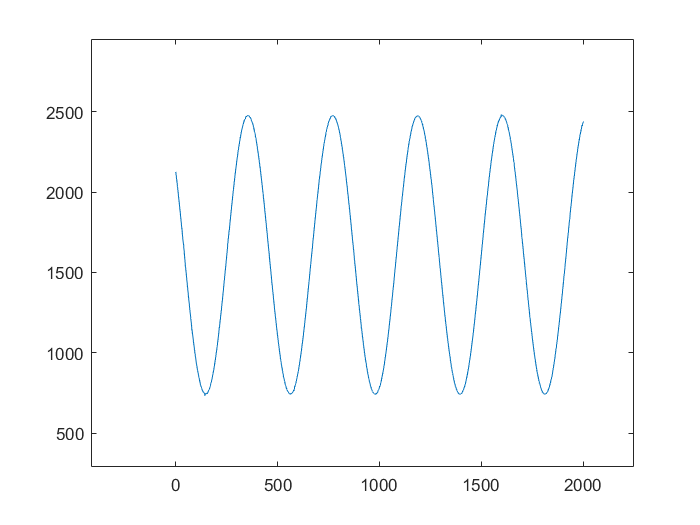
\includegraphics[width=\textwidth]{assets/exp4/onda2khz.png}
\caption{Plot dei dati ricevuti}
\end{figure}